
\section{Related Work}
Due to the popularity of the SGM, a lot of research went into optimizing it. This research can be divided into two categories, optimization of the throughput and the optimization of the algorithm's accuracy. The latter was achieved by allowing words to have multiple meanings, also called context-sensitive word embedings. For our work, the optimization of the throughput is of big interest while the semantic optimization is aimed at giving the reader a more holistic comprehension of the possible research directions.
This subsection will first give an overview of the optimization of the throughput and then present one paper that focused on context-sensitive word embeddings.

\subsection{Optimization of the throughput}

In the original model, the optimization is done with Stochastic Gradient Descent (SGD), which is a sequential algorithm. This process does not favor parallelization. To deal with this specific problem Mikolov et al.\cite{mikolov2} used a Hogwild tree proposed by Recht et al.\cite{hogwild}. The approach is to allow multiple threads to access a shared memory, in this case, the single model. In the original SGM, the threads are constructed as follows: at the beginning of training, the dataset is split into $N$ evenly sized chunks and each of these chunks will be processed by a one thread. The threads run parallel and have access to the shared memory. Therefore, overwriting errors are bound to happen. According to Recht et al.\cite{hogwild} the overwriting errors won't lead to a significant accuracy loss if the data is sparse enough. But in the case of NLP, the problem seems to be a bit more significant, and especially for word embedding, as many words share the same context words. There were several attempts at solving this issue, and we are going to cover a few of them in the following subsubsections.

\paragraph{Parallelization by the use of caching}
This idea was proposed by Vuurens et al. \cite{efficient}. The architecture used here is the basic skip gram model with a hierarchical softmax. The general idea is to cache the most frequently used nodes of the binary tree used to memorize the probability distribution and update them on the shared single model after a certain number of seen words (the paper used the number 10). The paper produced interesting results as they managed to decrease execution time by increasing the number of cores used for the calculation. This is very powerful because in the original implementation the execution time regressed after using more than 8 cores. It seems to indicate that too much overwriting was happening, as the number of concurrent threads surpasses a certain threshold. This can be seen in Figure \ref{fig:efficient}, where c31 is the model proposed by Vuurens et al.\cite{efficient}. The model did not suffer any accuracy loss in comparison to the original SGM model.
\begin{figure}[ht]
\centering
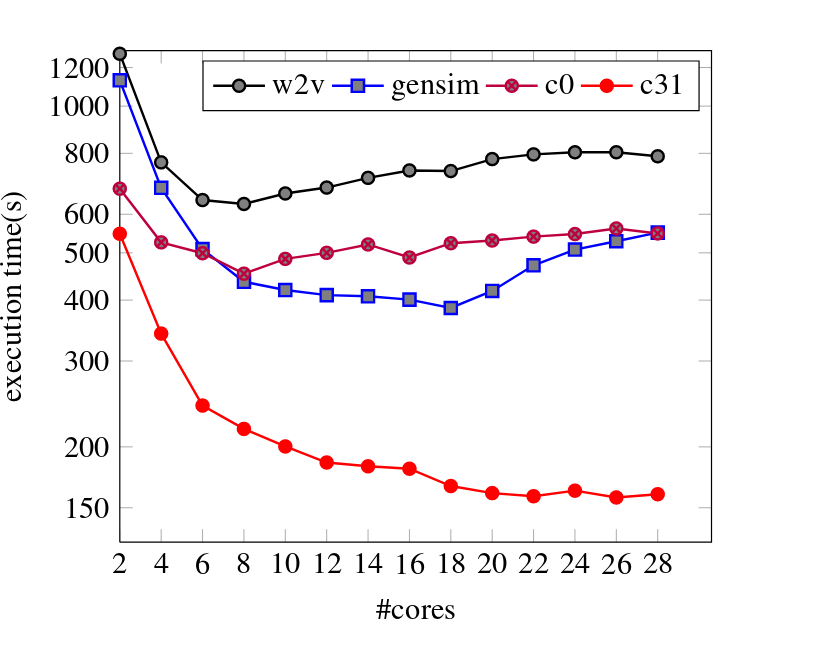
\includegraphics[scale=0.3]{images/cachingEfficiency.png}
\caption{Comparasion of the execution time in relation to the number of used cores \cite{efficient}}
\label{fig:efficient}
\end{figure}
This work proposes a very good way to parallelize the SGM, as in particular, it allows using more cores during the computation. As this approached focused on the Hierarchical softmax, in contrast to our work which used negative sampling, the next subsection covers optimizations of the Skip-Gram Model with negative sampling(SGNS).

\paragraph{Parallization in shared and Distributed Memory}
The first parallelized solution which was proposed by Ji et al. \cite{intel}, is to try to reduce the cost of our vector multiplication. The main idea in this paper is to convert the level 1-BLAS (Basic linear subprogram) vector to vector operations to a level 3-BLAS matrix multiplication operation, which are efficiently implemented into hardware and consequently faster. This is achieved, by using the same negative samples for each context word of a given word $w$. Instead of using for each context word a vector to vector multiplication we can transform this into a matrix multiplication, under the assumption that we will not lose accuracy by sharing the same negative samples. The matrix multiplication can be represented in the following way.
\[
\begin{bmatrix}
w \\
w_{n_1} \\
\vdots \\
w_{n_k}\\
\end{bmatrix}
*
\begin{bmatrix}
w_{c_1}\\
\vdots\\
w_{c_{2m}}\\
\end{bmatrix}
\]

where $w$ is our given word, $w_{n_1}...w_{n_k}$ are the shared negative samples, with $k \in [5,20]$, and $w_{c_1}...w_{c_2m}$ are the words inside of the context window $m$ of $w$, with $m \in [10,20]$, also called a batch of input context words. After each batch the model updates the weights of the used vectors.
This model achieves a 3.6 fold increase in throughput, by only losing 1\% of accuracy. An aspect that is not as useful to us is that the experiments were done on CPU, as modern GPU's are often used in many machine learning libraries, as with CUDA for example, there still need work to be done to optimize it with GPU's. This was done by Seulki and Youngmin \cite{gpu}, which is described in the next subsection.

\paragraph{Accelleration of word2vec by Using GPU's}
Seulki and Youngmin \cite{gpu} focused on getting a better throughput on the SGM when using GPU's. As the SGM is a sequential algorithm, is is not easy to parallelize it, especially if one wants to parallelize the training of individual training samples. As the algorithm goes sequentially over a sentence, the samples next to each other, in order of execution, will almost every time have the same input word. Consequently, it's very hard to parallelize at this level. To solve this problem, Seulki and Youngmin \cite{gpu} proposed the idea to parallelize the update of each dimension of the word embedding, since those are completely independent of each other. They achieved this by mapping each dimension to a CUDA thread while mapping each sentence to a CUDA block. As each CUDA block runs independently, the training of the sentences is parallelized, and the fact that sentences have different length is of no problem. If the execution time of the GPU kernel is greater than time used to read the sentences, it could be a smart choice to use multiple GPU's. According to Seulki and Youngmin \cite{gpu}, if multiple GPU's are used, there is a need for synchronizing the model, which will hinder run time performance. They achieved their best results with 2 concurrent GPU'S. The accomplished results were very good as they managed a 20x speedup compared to a single threaded CPU execution, which is a 3x increase in comparison to the original C code from Mikolov et al. \cite{mikolov2}, with no loss in accuracy. The problem with this and all the above optimization is that the code is not easily available. Therefore, we need an optimized implementation of the SGM that is easily available. This is provided by Gensim \cite{gensim}, which will be outlined in the next subsection.
%%%%%%%%%%%
\paragraph{Gensim}\label{ssec:gensim}
Gensim \cite{gensim} is a pure Python library that holds a state of the art implementation of the SGM. Gensim is written in Cython, which first allowed Gensim to have the same runtime as the original C code. Furthermore, it made use of BLAS's and precomputed sigmoid tables, while also trying to parallelize the training of different sentences. This finally yielded in a 4x speedup in run time. Gensim is an important tool as it allows us, as a python library, to compare our data rather easily. It was also used in related work \cite{intel} and is therefore of value, as it allows to us compare our work in a simpler way. This concludes our overview of the optimizations of the throughput of the SGM. In the next subsection, we give a quick outlook of what has been done in the field of context-sensitive word embeddings.

\subsubsection{Context sensitive word embedding}
A word has different meanings dependent on its context. This is a problem that is not addressed by the SGM. Some new models, that have taken this issue into consideration, were proposed. A lot of work has been done in this direction, Liu et al.\cite{topicalWE} and Bartunov et al.\cite{breaking} for example, but the one reporting the best results is Liu et al. \cite{contextWithTensor}. The concept of this approach is to change the way we compute the objective function and variables we use in our conditional probability. The idea is to look if a word given a certain context word matches to a topic. \textit{Bank} would match to \textit{finance} given the context word \textit{money}. \textit{Bank} would also match to \textit{nature} if \textit{river} was the given context word. But \textit{Bank} would not match to \textit{nature} with the context word \textit{money}. Now one could ask how to achieve such a context sensitive word embedding? First, we have to introduce new variables, therefore let's look at the objective function used:
\begin{equation}
J(\Omega) = \sum_{(w,t,c)\in D} \sum_{(w,\tilde{t},\tilde{c} \in{\tilde{D}})} max(0,1- g(w,t,c) + g(w,\tilde{t},\tilde{c})) \lambda||\Omega||_{2}^2
\end{equation}

This approach uses the same negative sample technique as described in the previous subsections, $D$ is the corpus data and $\tilde{D}$ is the set of negative samples and $\lambda$is the hyper parameter used for the standard $L_2$ standardization. What is interesting here is the function $g(w,c,t)$, where $w$ is a word, $c$ the context word, and $t$ the context in which the word appears. $g$ is defined as follows:
\begin{equation}
g(w,c,t) = u^T \sigma(w^TM^{[1:k]}t+V_c^T(w \oplus t) + b_c)
\end{equation}
where, $u, V_c, b_c$ are standard parameters for a neural network. $\oplus$ is the vector concatenation. The most important parameter is $M^{[1:k]}$, which is a tensor layer, the tensor layer is used because of its ability to model multiple interactions in the data, as this will be useful for multiple contexts. They used SGD for the optimization of this objective function. They achieved interesting results as shown in \ref{fig:multipleContext}.\\
\begin{figure}[ht]
\centering
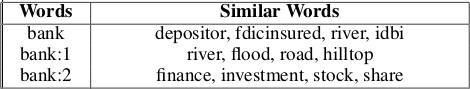
\includegraphics[scale=0.7]{images/multipleContext.png}
\caption{"Nearest neighbor words model and Skip-
Gram. The first line in each block is the results of Skip-Gram;
and the rest lines are the results of our model" \cite{contextWithTensor}}
\label{fig:multipleContext}
\end{figure}

This will conclude our overview of the related work. We will now give the reader an outline of the different Gradient Descent Optimizer used in our experiments.